\section{Objective}
\label{sec:Objective}

The objective of this lab course is to understand the basic concepts of scintillating fibers.
This is achieved by measuring different aspects of the light propagation inside the fibers and comparing the results
with simulated data.

\section{Theory}
\label{sec:Theory}

In detectors for high energy particle physics, a precise track reconstruction is crucial to succefully reconstruct collision events.
There are many different solutions to realising such a tracking detector, each with their own advantages and disadvanteges, for example
in regard to their resolution, size, cost. Scintilators are one type of such a tracking detector, used as an example by the famous
LHCb experiment. If charged particles pass through a scintillator, photons are emmited that can be measured. The following section will explain
how a tracking detector can be constructed using this principle.

\subsection{Scintilating fibre trackers}

A tracker is constructed by using many individual scintillating fibres. If a charged particle passes through one of these fibers, photons are produced that
travel towards the end of the fiber, where they can be detected. The main advanteges of this type of tracker is its high resolution, as the fibers can
be constructed rather thin (\qty{250}{\micro\meter} in LHCb). Penetrating particles are scattered less in the fibres compared to other methods,
so the error introduced by the detector is kept low. Lastly, these fibres are inexpensive, so a large surface can be covered which increases
the sensitivity of the detector \cite{SciFi}.
The single fibres are combined into fibre mats, by arranging them in a hexagonal pattern to minimize uncovered area and glueing
them together using an epoxy. A cross section of this arrangment can be seen in \autoref{fig:fibre-mats}.

\begin{figure}[H]
	\centering
	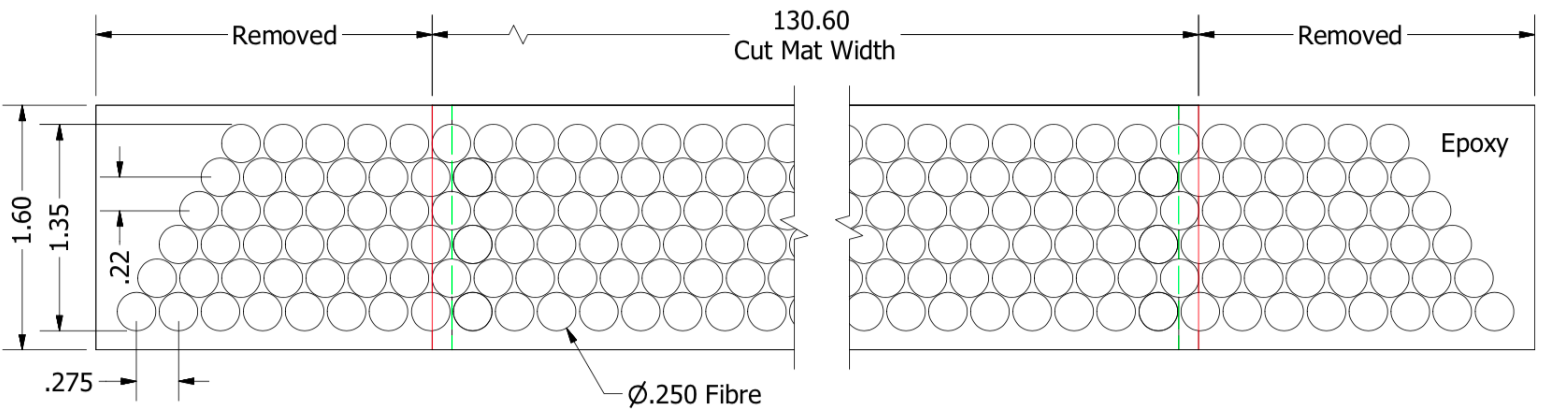
\includegraphics[width=0.9\linewidth]{pics/fibre_mat.png}
	\caption{Cross section of the fibre mat constructed out of the scintillating fibres \cite{SciFi}.}
	\label{fig:fibre-mats}
\end{figure}

In case of the LHCb detector four layers, each consisting of 40 mats, are positioned behind each other. The middle layers are tilted by \qty{5}{\degree}
to allow a spacial resolution in the entire plane perpendicular to the beam pipe.

The photons created by the scintillations travel to the ends of the fibres and are detected there using silicon photomultipliers.
These consit of avalanche photodiodes, where each diode represents a pixel. If a photon hits a pixel, an electron-hole pair is created
in the diode. Due to an applied high voltage, the electrons are accelerated and trigger more electron-hole pairs to form.
Consequentlly, a charge avalanche is registered in form of a current pulse. After a short recovery time, the pixel is ready to sense another signal.
The silicon photomultipliers cannot detect all incoming photons, they have a photodetection efficiency depending on the wavelenth of
the photons. At the optimal wavelength, approximatly \qty{43}{\percent} of photons are detected. The silicon photomultipliers themselves
are not sensitive to the wavelenth of the light and thus measure an effective attenuation over all wavelengths. Lastly, there will
always be a certain noise within the pixels leading to the presence of a dark current, even if no photons hit the pixel.

\subsection{Scintillating fibres}

In the following, the internal structure of the scintillating fibres will be explained. Additionally, some important
arguments about how the light propagates inside the fibers is given.

\subsubsection{Structure of scintillating fibres}

The core of the fibres consits of a \qty{220}{\micro\meter} thick polystyrene core. This is an organic scintillator,
meaning that the scintillations caused by charged particles are based on a molecular processes. If a charged particle
passes through the fibre, valence electrons of the polystyrene are excited. During the relaxation process, UV photons
are emmited and travel through the fibre. To ensure that the photons remain inside the fiber, the outer layers are chosen
in a way to allow total internal reflection to occur. This is archieved by surrounding the core with two sheaths with
outwardly decreasing refractive indices. Both sheats have a thickness of \qty{7.5}{\micro\meter}, resulting in a total fibre width
of \qty{250}{\micro\meter}. A basic sktech of this fibre layout can be seen in \autoref{fig:fibre}.

\begin{figure}[H]
	\centering
	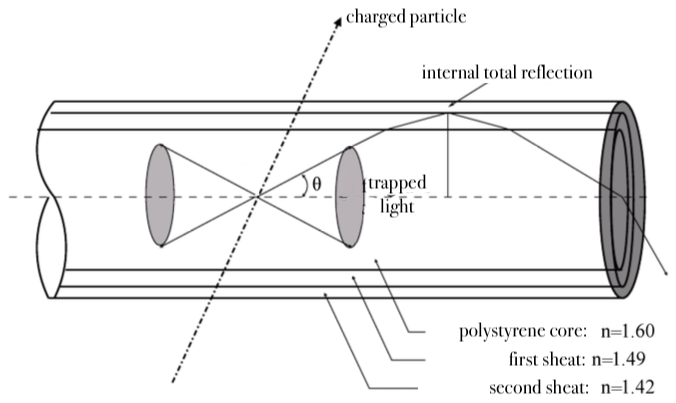
\includegraphics[width=0.7\linewidth]{pics/fibre.png}
	\caption{Schematic structure of the scintillating fibre used in the experiment \cite{SciFi}.}
	\label{fig:fibre}
\end{figure}

The refractive indices are also given in \autoref{fig:fibre}, it can easily be seen that they decrease towards the outside
of the fibre. This ensures proper propagation of the photons discussed in the next chapter.

\subsubsection{Photon propagation in the fibres}

Since the UV photons will always be emmited at a distance $r_\text{min}$ towards the center of the fibre and with a given angle $\theta$,
reflections at the first and second sheat will occur. This is visualized in \autoref{fig:photon_path}.

\begin{figure}[H]
	\centering
	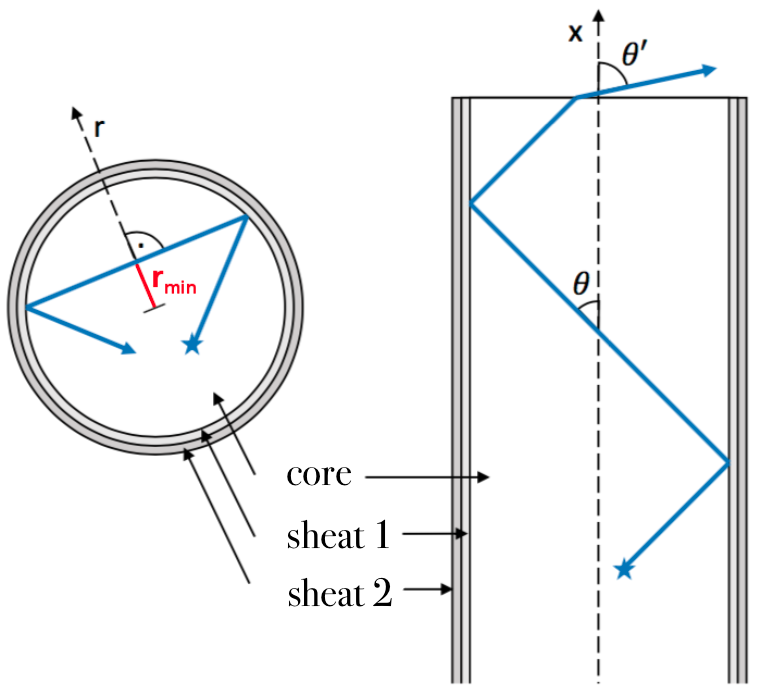
\includegraphics[width=0.5\linewidth]{pics/photon_path.png}
	\caption{Path of a photon trough the scintillating fibre \cite{SciFi}.}
	\label{fig:photon_path}
\end{figure}

Assuming that the photon remains inside the core, the path length of the photon $L$ and the number of
times it reflects $N$ are given by
\begin{align}
    L &= \frac{x}{\cos{\theta}} \, , \label{eq:L} \\ 
    N &= \frac{x \tan{\theta}}{2 \sqrt{r_\text{core}^2-r_\text{min}^2}} \, \label{eq:N} .
\end{align}
Here, $r_\text{core}^2$ is the radius of the fibre core and $x$ is the distance to the fibre end.
The angle towards the inteface $\theta_\text{refl}$ at the end of the fibre can be calculated using the formula
\begin{align*}
    \theta_\text{refl} &= \arcsin{\sqrt{1-\frac{r_\text{min}^2}{r_\text{core}^2}} \sin{\theta}} .
\end{align*}
Some of the photons travelling inside the fibre are lost due to different processes. This is why
the fibre has a specific capture efficiency that describes what fraction of photons remain inside it.
Photons can undergo Raygleigh scattering with the fibre material or be absorbed by it. In general, the attentuation $I$
of photons after traveling a distance $L$ in the fiber exponentially decreases according to
\begin{equation*}
    I(x) = I_0 \exp{\left(-\frac{L}{\Lambda}\right)} = I_0 \exp{\left(- a L \right)} \, ,
\end{equation*}
where $\Lambda$ is the attentuation length which is approximatly \qty{3.5}{\metre} in the fibers used for this experiment.
The inverse attentuation length $a$ is called the attenuation coefficient.
To further parameterize the photon attentuation, it is useful to differentiate between losses due to the core material
$A_\text{core}$ and losses due to reflection $A_\text{refl}$. Now the total attentuation can be expressed as
\begin{equation}
    I(x, \theta) = I_0 A_\text{core}(x, \theta) A_\text{refl}(x, \theta) .
    \label{eq:I}
\end{equation}
Losses in the core material depend exponentially on the path length of the photon via
\begin{equation}
    A_\text{core}(x, \theta) = \exp{\left(-\frac{L(x, \theta)}{\Lambda}\right)} .
    \label{eq:core}
\end{equation}
For reflection losses, the number of reflections $N$ and probability of loss during reflection $\varepsilon$ is needed.
In this case, the losses also show an exponential dependance on these parameters:
\begin{equation}
    A_\text{refl}(x, \theta) = \exp{\left(- \varepsilon N(x, \theta)\right)} .
    \label{eq:refl}
\end{equation}
Now, relations \eqref{eq:core} and \eqref{eq:refl} can be inserted into \eqref{eq:I}. Lastly, the known expressions
for $L(x, \theta)$ \eqref{eq:L} and $N(x, \theta)$ \eqref{eq:N} can be used to obtain the final formula
\begin{equation}
    I(x, \theta) = I_0 \exp{ \left( -x \underbrace{\left(\frac{1}{\cos{\theta}} + \frac{\varepsilon \tan{\theta}}{2 \sqrt{r_\text{core}^2-r_\text{min}^2}} \right)}_{a_\text{eff}} \right)} .
    \label{eq:Attentuation}
\end{equation}
Here, $a_\text{eff}$ summarizes the parameters as the effective attentuation coefficient.